\section{Estatísticas Gerais}

Nesta seção, são apresentadas as estatísticas gerais dos dados coletados para os dispositivos Smart TV e Chromecast, sem considerar o horário em que os dados foram gerados. As análises incluem cálculos de medidas descritivas, como média, variância e desvio padrão, além de representações gráficas através de histogramas, boxplots e funções de distribuição empírica (ECDF). 

\subsection{Medidas Descritivas}

As medidas descritivas para as taxas de upload e download (em escala logarítmica base 10) estão resumidas na Tabela~\ref{tab:estatisticas}. Para determinar o número adequado de bins para os histogramas, utilizamos a fórmula de Sturges:

\begin{equation}
k = 1 + \log_2(n),
\end{equation}

onde \(n\) é o número total de amostras. Este método busca otimizar a visualização dos dados ao balancear granularidade e clareza.

\begin{table}[H]
\centering
\caption{Medidas descritivas das taxas de upload e download.}
\label{tab:estatisticas}
\begin{tabular}{|c|c|c|c|}
\hline
\textbf{Dispositivo} & \textbf{Tipo de Tráfego} & \textbf{Média} & \textbf{Desvio Padrão} \\ \hline
Smart TV & Upload & 2.16 & 2.03 \\ \hline
Smart TV & Download & 2.35 & 2.59 \\ \hline
Chromecast & Upload & 3.35 & 0.68 \\ \hline
Chromecast & Download & 3.80 & 1.29 \\ \hline
\end{tabular}
\end{table}

O número de bins calculado para cada dispositivo, arredondando para cima, é o seguinte:
\begin{itemize}
    \item \textbf{Smart TV:} \(k = 24\) bins.
    \item \textbf{Chromecast:} \(k = 22\) bins.
\end{itemize}

\subsection{Visualizações Gráficas}

Para compreender melhor a distribuição dos dados, utilizamos as seguintes representações gráficas:

\begin{itemize}
    \item \textbf{Histogramas:} As distribuições das taxas de upload e download para cada dispositivo estão representadas nos histogramas da Figura~\ref{fig:histogramas}.
    \item \textbf{Boxplots:} A Figura~\ref{fig:boxplots} mostra os boxplots comparando as taxas de upload e download entre Smart TV e Chromecast.
    \item \textbf{ECDF:} As funções de distribuição empírica, exibidas na Figura~\ref{fig:ecdf}, demonstram a probabilidade acumulada para cada valor das taxas.
\end{itemize}

\begin{figure}[H]
    \centering
    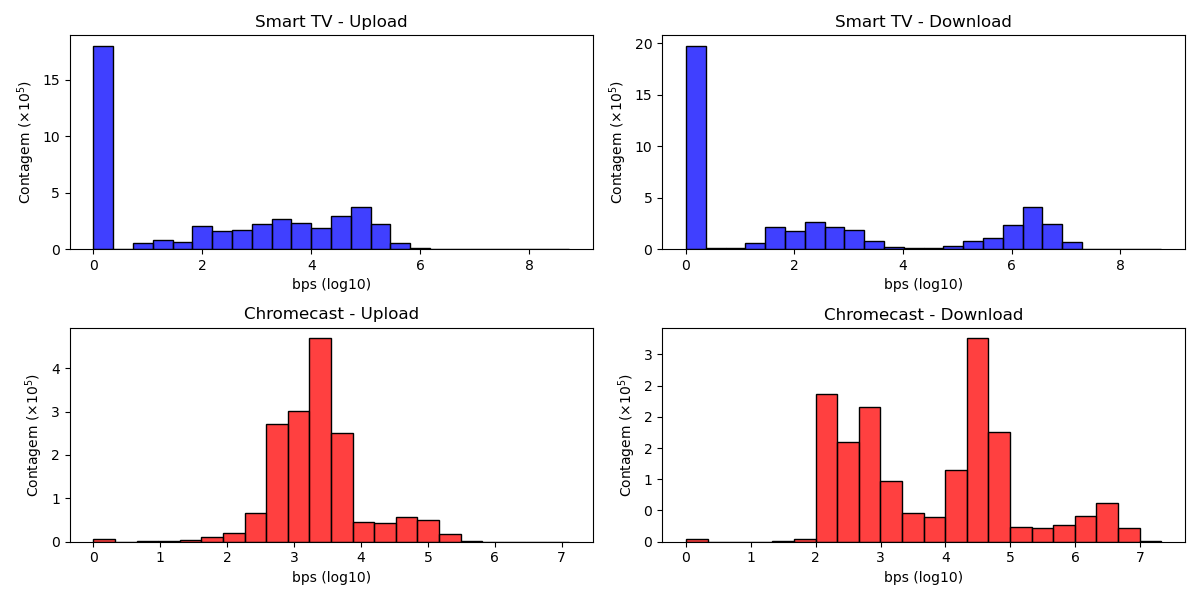
\includegraphics[width=0.8\textwidth]{../estatísticas gerais/histogramas.png}
    \caption{Histogramas das taxas de upload e download para Smart TV e Chromecast.}
    \label{fig:histogramas}
\end{figure}

\begin{figure}[H]
    \centering
    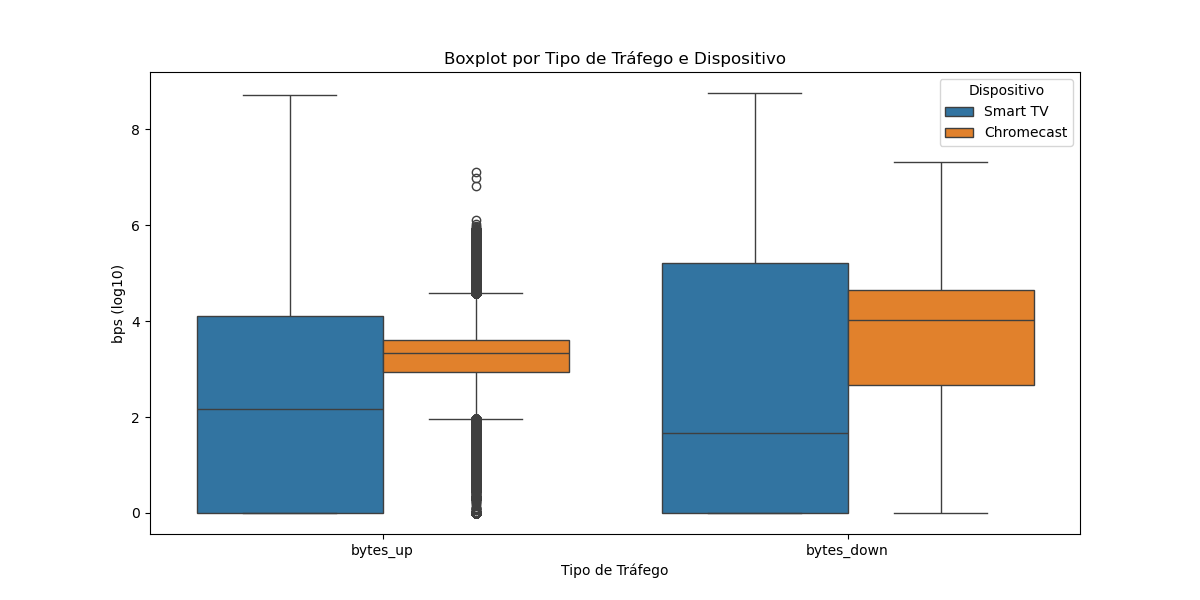
\includegraphics[width=0.8\textwidth]{../estatísticas gerais/boxplot.png}
    \caption{Boxplots das taxas de upload e download para Smart TV e Chromecast.}
    \label{fig:boxplots}
\end{figure}

\begin{figure}[H]
    \centering
    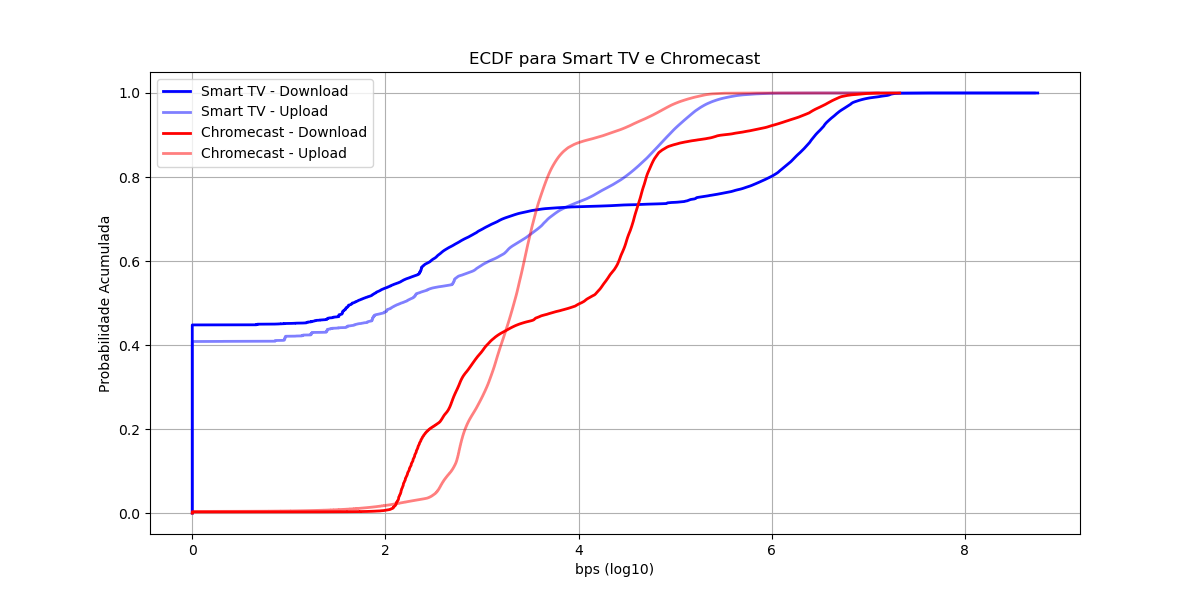
\includegraphics[width=0.8\textwidth]{../estatísticas gerais/ecdf.png}
    \caption{Funções de Distribuição Empírica (ECDF) das taxas de upload e download.}
    \label{fig:ecdf}
\end{figure}

\subsection{Análise dos Resultados}

Os resultados indicam que as taxas de upload e download apresentam características distintas entre os dispositivos:
\begin{itemize}
    \item \textbf{Smart TV:} As taxas exibem maior variação, refletida em desvios padrão mais elevados. 
    \item \textbf{Chromecast:} As taxas são mais concentradas, indicando menor dispersão nos valores.
\end{itemize}

Essas diferenças podem ser atribuídas aos diferentes padrões de uso e capacidades técnicas dos dispositivos, como consumo contínuo em Smart TVs e interações esporádicas em Chromecasts.
